\chapter{Apriori: Assoziationsregeln}
\label{chap:apriori}

\begin{myremark}[Algorithmusart in diesem Kapitel]
    Funktionsart: \textbf{Assoziation}. \\
    Umsetzungsart: \textbf{selbstlernend}.
\end{myremark}

\begin{myremark}
    Dieses Kapitel zeigt ein anderes Ziel als Klassifikation oder Regression:
    Wir suchen nicht primär eine Vorhersage, sondern \textbf{häufige Muster} und \textbf{Regeln}
    in Transaktionsdaten.
\end{myremark}

\section{Grundidee: Von häufigen Itemsets zu Regeln}

\begin{mydefinition}[Apriori]
    Der \textbf{Apriori-Algorithmus} kann verwendet werden, um gewisse Dinge in Daten zu entdecken, die oft zusammen auftreten. Zum Beispiel in einem Supermarkt, um in den Daten von Warenkörben (oder ähnlichen Datensätzen) häufige Kombinationen von Produkten zu finden. Diese Kombinationen nennen wir \textbf{Itemsets}. Wenn wir wissen, dass bestimmte Produkte oft zusammen gekauft werden, können wir daraus \textbf{Assoziationsregeln} wie \enquote{Wenn jemand Brot und Butter kauft, kauft er oft auch Milch} ableiten.

    Die Kernidee lautet: Wenn ein Itemset häufig ist, dann sind auch alle seine Teilmengen häufig.
    Umgekehrt gilt: Ist eine Teilmenge nicht häufig, kann keine Obermenge häufig sein.

    Der Algorithmus funktioniert iterativ:
    \begin{enumerate}
        \item \textbf{Minimum Support Threshold}: Zuerst wird ein sogenannter minimaler Support festgelegt, der angibt, wie oft ein Itemset in den Daten vorkommen muss, um als häufig zu gelten.
        \item \textbf{Frequent Itemset Mining}: Der Algorithmus beginnt mit der Suche nach häufigen Itemsets der Grösse 1 (also einzelnen Items). Hierzu wird der Support jedes einzelnen Items berechnet und mit dem Schwellenwert verglichen. Alle Items, die den Mindest-Support erfüllen, werden als häufige Itemsets der Grösse 1 betrachtet.
        \item \textbf{Kandidaten generieren}: Aus den häufigen Itemsets der Grösse $k$ werden Kandidaten für häufige Itemsets der Grösse $k+1$ generiert. Dies geschieht durch die Kombination von häufigen Itemsets, die sich nur in einem Item unterscheiden.
        \item \textbf{Support berechnen}: Für die generierten Kandidaten wird der Support berechnet, und diejenigen, die den Mindest-Support erfüllen, werden als häufige Itemsets der Grösse $k+1$ betrachtet.
        \item \textbf{Regeln ableiten}: Sobald alle häufigen Itemsets gefunden wurden, können Assoziationsregeln abgeleitet werden. Eine Regel hat die Form \enquote{Wenn $X$ dann $Y$}, wobei $X$ und $Y$ Itemsets sind. Für jede Regel werden Kennzahlen wie Support, Confidence und Lift berechnet, um die Stärke der Regel zu bewerten.
    \end{enumerate}
\end{mydefinition}




Zur Erklärung der Mengennotation:
\begin{itemize}
    \item \textcolor{ForestGreen}{X} ist die Menge aller Transaktionen, die $X$ enthalten.
    \item \textcolor{ForestGreen}{$P(X)$} ist der Anteil aller Transaktionen, die $X$ enthalten.
    \item \textcolor{blue}{$P(Y)$} ist der Anteil aller Transaktionen, die $Y$ enthalten.
    \item \textcolor{red}{$P(X \cup Y)$} ist der \emph{Anteil} dieser Transaktionen als Bruchteil der Gesamtzahl aller Transaktionen.
    \item \textcolor{orange}{$P(X \cap Y)$} (gelesen: \enquote{$X$ geschnitten $Y$}) ist der Anteil aller Transaktionen, die sowohl $X$ als auch $Y$ enthalten.
\end{itemize}

\begin{center}
    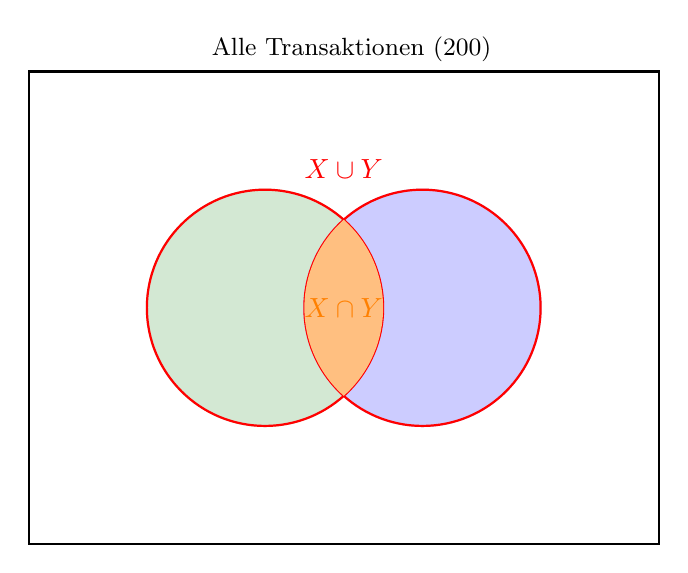
\begin{tikzpicture}[
            filled/.style={fill=red!20, draw=red!20, thick},
            outline/.style={draw=red!80, thick}
        ]
        % Zwei Kreise mit Überlappung
        % \draw[filled] (0,0) circle (1.5) node {$X$} (2,0) circle (1.5) node {$Y$};
        \draw[fill=ForestGreen!20, draw=ForestGreen!20, thick] (0,0) circle (1.5);
        \draw[fill=blue!20, draw=blue!20, thick] (2,0) circle (1.5);
        % outline union
        \draw[thick, red] (0,0) circle (1.5);
        \draw[thick, red] (2,0) circle (1.5);
        \node[anchor=south] at (current bounding box.north) {\textcolor{red}{$X \cup Y$}};
        % show intersection in orange
        \begin{scope}
            \clip (0,0) circle (1.5);
            \fill[orange!50] (2,0) circle (1.5);
        \end{scope}
        \node at (1,0) {\textcolor{orange}{$X \cap Y$}};

        % Rechteck für Universalmenge
        \draw[thick] (-3,-3) rectangle (5,3);
        \node[anchor=south east] at (3,3) {\small Alle Transaktionen (200)};
    \end{tikzpicture}
\end{center}

In Realität könnte es sein, dass $P(X \cup Y)$ nicht gleich $P(X) \cdot P(Y)$ ist, weil $X$ und $Y$ nicht unabhängig sind. Es könnte beispielsweise sein, dass $X$ und $Y$ oft zusammen auftreten, was zu einem höheren $P(X \cup Y)$ führt als erwartet. In diesem Fall wäre die Regel \enquote{Wenn $X$ vorkommt, tritt oft auch $Y$ auf} besonders interessant, da sie auf eine starke Assoziation zwischen den beiden Items hinweist.

\begin{mydefinition}[Support, Confidence, Lift]
    Für eine Regel \enquote{$X \Rightarrow Y$}, also \enquote{Wenn $X$ vorkommt, tritt oft auch $Y$ auf}, gibt es drei wichtige Kennzahlen:

    \begin{itemize}
        \item \textbf{Support} misst, wie häufig die Kombination \textcolor{red}{$X \cup Y$} in den Transaktionen vorkommt:
              \[
                  \text{Support}(X \Rightarrow Y) = P(X \cup Y)
              \]
        \item \textbf{Confidence} misst, wie wahrscheinlich \textcolor{blue}{$Y$} ist, wenn \textcolor{ForestGreen}{$X$} bereits vorhanden ist (also die relative Häufigkeit von \textcolor{orange}{$X \cap Y$} innerhalb von \textcolor{ForestGreen}{$X$}).

              \[
                  \text{Confidence}(X \Rightarrow Y) = \frac{P(X \cup Y)}{P(X)}
              \]
        \item \textbf{Lift} misst, wie viel häufiger \textcolor{blue}{$Y$} in Transaktionen mit \textcolor{ForestGreen}{$X$} vorkommt, verglichen mit der Erwartung, wenn \textcolor{ForestGreen}{$X$} und \textcolor{blue}{$Y$} unabhängig wären (also die Häufigkeit von \textcolor{orange}{$X \cap Y$} im Vergleich zum Produkt der Häufigkeiten von \textcolor{ForestGreen}{$X$} und \textcolor{blue}{$Y$}).

              \[
                  \text{Lift}(X \Rightarrow Y) = \frac{P(X \cup Y)}{P(X)\,P(Y)}
              \]
    \end{itemize}
\end{mydefinition}

\begin{myexample}[Apriori-Algorithmus]
    Angenommen, wir haben einen Datensatz von 200 Transaktionen in einem Supermarkt, und wir möchten herausfinden, welche Produkte oft zusammen gekauft werden. Wir setzen einen \textbf{Mindest-Support von 20\%} fest, was bedeutet, dass ein Itemset in mindestens 40 Transaktionen vorkommen muss, um als häufig zu gelten.

    Der Datensatz enthält die folgenden Informationen:
    \begin{table}[H]
        \centering
        \begin{tabular}{c|c}
            \textbf{Transaktion} & \textbf{Produkte}          \\
            \midrule
            1                    & Brot, Butter, Milch        \\
            2                    & Brot, Windeln, Bier, Eier  \\
            3                    & Milch, Windeln, Bier, Cola \\
            4                    & Brot, Milch, Windeln, Bier \\
            5                    & Brot, Milch, Windeln, Cola \\
            ...                  & ...                        \\
            200                  & ...                        \\
        \end{tabular}

        \caption{Beispielhafte Transaktionsdaten}
    \end{table}
    Zunächst berechnen wir den Support für einzelne Items:
    \begin{table}[H]
        \centering
        \begin{tabular}{l|c|c|l}
            \textbf{Item} & \textbf{Support Count} & \textbf{Support} \% &                                                             \\
            \midrule
            Brot          & 100                    & 50\%                & \multirow{4}{*}{\textcolor{ForestGreen}{> Mindest-Support}} \\
            Milch         & 80                     & 40\%                &                                                             \\
            Windeln       & 60                     & 30\%                &                                                             \\
            Bier          & 50                     & 25\%                &                                                             \\\midrule\midrule
            Butter        & 30                     & 15\%                & \multirow{4}{*}{\textcolor{red}{< Mindest-Support}}         \\
            Cola          & 20                     & 10\%                &                                                             \\
            Eier          & 10                     & 5\%                 &                                                             \\
        \end{tabular}
        \caption{Support Count und Support \% der einzelnen Items}
    \end{table}
    In diesem Fall sind die häufigen \textbf{Itemsets der Grösse 1}: \{Brot, Milch, Windeln, Bier\}.

    Als nächstes generieren wir Kandidaten für \textbf{Itemsets der Grösse 2}, z.B. \{Brot, Milch\}, \{Brot, Windeln\}, \{Milch, Windeln\}, \{Brot, Bier\}, etc.:

    \begin{table}[H]
        \centering
        \begin{tabular}{l|c|c|l}
            Itemset            & Support Count & Support \% &                                                             \\
            \midrule
            \{Brot, Milch\}    & 50            & 25\%       & \multirow{2}{*}{\textcolor{ForestGreen}{> Mindest-Support}} \\
            \{Brot, Windeln\}  & 40            & 20\%       &                                                             \\\midrule\midrule
            \{Milch, Windeln\} & 30            & 15\%       & \multirow{3}{*}{\textcolor{red}{< Mindest-Support}}         \\
            \{Brot, Bier\}     & 25            & 12.5\%     &                                                             \\
            ...                & ...           & ...        &                                                             \\
        \end{tabular}
        \caption{Support Count und Support \% der Itemsets der Grösse 2}
    \end{table}

    Wir berechnen den Support für diese Kandidaten und behalten nur diejenigen, die den Mindest-Support von 20\% erfüllen. Angenommen, \{Brot, Milch\} kommt in 50 Transaktionen vor (25\%), \{Brot, Windeln\} in 40 Transaktionen (20\%), \{Milch, Windeln\} in 30 Transaktionen (15\%), \{Brot, Bier\} in 25 Transaktionen (12.5\%), etc. In diesem Fall wären die häufigen Itemsets der Grösse 2: \{Brot, Milch\}, \{Brot, Windeln\}.

    Schliesslich können wir aus diesen häufigen Itemsets \textbf{Regeln} ableiten, z.B. \enquote{Wenn Brot, dann Milch}, und die entsprechenden Kennzahlen berechnen, um die Stärke der Regel zu bewerten. Obschon Brot und Windeln häufig zusammen gekauft werden, könnte es sein, dass dies lediglich daran liegt, dass beide Produkte einzeln häufig gekauft werden (und daher zufälligerweise auch recht häufig zusammen), ohne dass eine starke Assoziation zwischen ihnen besteht. Daher ist es wichtig, die Confidence und den Lift zu berechnen, um die Qualität der Regel zu beurteilen.

    Dies wird gemacht, indem wir die \textbf{Confidence} (wie oft Milch gekauft werden, wenn Brot gekauft wird) berechnen. Hierzu legen wir eine \textbf{Schwelle für die Confidence fest, z.B. 70\%}, um zu entscheiden, ob die Regel als stark genug gilt, um weiterverwendet zu werden.

    \begin{itemize}
        \item \textbf{Support} von \{Brot, Milch\} = 25\% (50 Transaktionen enthalten beide)
        \item \textbf{Support} von \{Brot\} = 50\% (100 Transaktionen enthalten Brot)
        \item \textbf{Confidence} von \enquote{Wenn Brot, dann Milch} = Support(\{Brot, Milch\}) / Support(\{Brot\}) = 25\% / 50\% = 50\%
    \end{itemize}
    In diesem Fall würde die Regel \enquote{Wenn Brot, dann Milch} eine Confidence von 50\% haben, was unter der Schwelle von 70\% liegt, und daher nicht als starke Regel betrachtet werden würde.

    Eine starke Regel könnte folgendermassen aussehen:
    \begin{itemize}
        \item \textbf{Support} von \{Brot, Butter\} = 40\% (80 Transaktionen enthalten beide)
        \item \textbf{Support} von \{Brot\} = 50\% (100 Transaktionen enthalten Brot)
        \item \textbf{Confidence} von \enquote{Wenn Brot, dann Butter} = Support(\{Brot, Butter\}) / Support(\{Brot\}) = 40\% / 50\% = 80\%
    \end{itemize}

    Um die Regelqualität weiter zu bewerten, könnte auch der \textbf{Lift} berechnet werden, um zu sehen, ob die Kombination von Brot und Butter tatsächlich eine stärkere Assoziation mit Brot hat als erwartet, wenn sie unabhängig wären:

    \begin{itemize}
        \item \textbf{Support} von \{Butter\} = 15\% (30 Transaktionen enthalten Butter)
        \item \textbf{Lift} von \enquote{Wenn Brot, dann Butter} = Support(\{Brot, Butter\}) / (Support(\{Brot\}) * Support(\{Butter\})) = 40\% / (50\% * 15\%) = 40\% / 7.5\% = 5.33
    \end{itemize}

    Ein Lift von 5.33 bedeutet, dass die Kombination von Brot und Butter 5.33-mal häufiger vorkommt, als wenn sie unabhängig wären, was auf eine sehr starke Assoziation zwischen den beiden Produkten hinweist.
\end{myexample}

\begin{myexercise}[Apriori-Algorithmus anhand gegebener Werte anwenden]
    Sie haben ausgewertet, welche Musik-Stile in Ihrer Klasse gehört werden:
    \begin{table}[H]
        \centering
        \begin{tabular}{c|c|c|c|c|c|c|c|c||c}
            \textbf{Person} & \textbf{Pop} & \textbf{Rock} & \textbf{Jazz} & \textbf{HipHop} & \textbf{Elektro} & \textbf{Klassik} & \textbf{Metal} & \textbf{Reggae} & $\Sigma$ \\
            \midrule\midrule
            1               & 1            & 1             & 0             & 1               & 0                & 0                & 0              & 1               & 4        \\\midrule
            2               & 1            & 0             & 0             & 1               & 1                & 0                & 0              & 0               & 3        \\\midrule
            3               & 0            & 1             & 1             & 0               & 0                & 0                & 1              & 0               & 3        \\\midrule
            4               & 1            & 1             & 0             & 0               & 1                & 0                & 0              & 0               & 3        \\\midrule
            5               & 1            & 0             & 1             & 0               & 0                & 1                & 0              & 0               & 3        \\\midrule
            6               & 0            & 1             & 0             & 1               & 1                & 0                & 0              & 0               & 3        \\\midrule
            7               & 1            & 0             & 0             & 1               & 0                & 0                & 0              & 1               & 3        \\\midrule
            8               & 0            & 1             & 1             & 0               & 0                & 1                & 0              & 0               & 3        \\\midrule
            9               & 1            & 1             & 0             & 1               & 0                & 0                & 1              & 0               & 4        \\\midrule
            10              & 0            & 0             & 1             & 0               & 1                & 1                & 0              & 0               & 3        \\\midrule
            11              & 1            & 1             & 0             & 0               & 0                & 0                & 1              & 0               & 3        \\\midrule
            12              & 0            & 0             & 0             & 1               & 1                & 0                & 0              & 1               & 3        \\\midrule
            13              & 1            & 0             & 1             & 0               & 0                & 0                & 0              & 1               & 3        \\\midrule
            14              & 0            & 1             & 0             & 1               & 0                & 1                & 0              & 0               & 3        \\\midrule
            15              & 1            & 0             & 0             & 0               & 1                & 0                & 1              & 0               & 3        \\\midrule
            \midrule\midrule
            $\Sigma$        & 9            & 8             & 5             & 7               & 6                & 4                & 4              & 4               & 47       \\
        \end{tabular}
        \caption{Musik-Stile der ganzen Klasse (15 Personen, 8 Stile; 1 = hört den Stil)}
    \end{table}
    Berechnen Sie die häufigen Itemsets der Grösse 1 und 2 mit einem Mindest-Support von 30\%, und leiten Sie daraus eine Regel ab, z.B. \enquote{Wenn jemand Pop hört, hört er oft auch Elektro}. Berechnen Sie die Kennzahlen Support, Confidence und Lift für diese Regel. Verwenden Sie einen Confidence-Schwellenwert von 70\%, um zu entscheiden, ob die Regel als stark genug gilt.

    \begin{myanswer}
        \textbf{Häufige Itemsets der Grösse 1:} Mit Mindest-Support von 30\% (mindestens 4.5, also 5 Personen) sind folgende Stile häufig:
        Pop (9), Rock (8), HipHop (7), Elektro (6), Jazz (5). Klassik, Metal und Reggae erfüllen den Schwellenwert nicht.

        \textbf{Häufige Itemsets der Grösse 2:} Für die Regel Pop $\Rightarrow$ Elektro:
        Personen, die beide hören: 2, 4, 15 $\Rightarrow$ 3 Personen. Dies entspricht 20\% und liegt unter dem Mindest-Support von 30\%, daher ist dies kein häufiges Itemset.

        \textbf{Regel Pop $\Rightarrow$ Elektro:}
        \begin{itemize}
            \item \textbf{Support} = $\frac{3}{15} = 0.20$ (20\%)
            \item \textbf{Confidence} = $\frac{3}{9} = 0.33$ (33\%)
            \item \textbf{Lift} = $\frac{0.20}{0.6 \cdot 0.4} = \frac{0.20}{0.24} = 0.83$
        \end{itemize}

        Diese Regel ist \textbf{nicht stark genug}, da die Confidence (33\%) deutlich unter dem Schwellenwert von 70\% liegt. Der Lift von 0.83 zeigt sogar, dass Pop und Elektro schwächer zusammenhängen, als wenn sie unabhängig wären.
    \end{myanswer}

\end{myexercise}

\begin{myexercise}[Kennzahlen berechnen]
    Ein Shop hat 200 Transaktionen:
    \begin{itemize}
        \item In 50 Transaktionen sind \enquote{Pasta} und \enquote{Tomatensauce} gemeinsam enthalten.
        \item \enquote{Pasta} kommt in 80 Transaktionen vor.
        \item \enquote{Tomatensauce} kommt in 70 Transaktionen vor.
    \end{itemize}
    Berechnen Sie für die Regel
    \enquote{Pasta $\Rightarrow$ Tomatensauce}:
    \begin{enumerate}
        \item Support
        \item Confidence
        \item Lift
    \end{enumerate}

    Interpretieren Sie die Ergebnisse unter der Annahme, dass Sie einen Mindest-Support von 20\% und eine Mindest-Confidence von 60\% festgelegt haben.
    \begin{myanswer}
        \begin{itemize}
            \item Support $= \frac{50}{200}=0.25$. \\
            \item Confidence $= \frac{50}{80}=0.625$. \\
            \item Lift $= \frac{0.25}{0.4\cdot0.35}=1.79$ (deutlich über 1).
        \end{itemize}
        Die Regel \enquote{Pasta $\Rightarrow$ Tomatensauce} erfüllt sowohl den Mindest-Support von 20\% als auch die Mindest-Confidence von 60\%. Der Lift von 1.79 zeigt, dass Pasta und Tomatensauce deutlich häufiger zusammen gekauft werden, als wenn sie unabhängig wären, was auf eine starke Assoziation zwischen den beiden Produkten hinweist.
    \end{myanswer}
\end{myexercise}

\section{Warum Schwellenwerte wichtig sind}

\begin{mycaution}
    Ohne sinnvolle Grenzwerte (z.\,B. \texttt{min\_support}, \texttt{min\_confidence})
    produziert Apriori sehr viele triviale oder zufällige Regeln.
    Das führt schnell zu \textbf{Scheinkorrelationen}.
\end{mycaution}

\begin{myexercise}[Regelqualität bewerten]
    Ein Data-Team meldet die Regel:
    \enquote{Energy-Drink $\Rightarrow$ Kopfhörer},
    Confidence $= 0.82$, aber Support $= 0.01$.
    \begin{enumerate}
        \item Wie könnten diese Kennzahlen zustande kommen? Was könnte dahinterstecken?
        \item Warum ist diese Regel trotz hoher Confidence kritisch zu prüfen?
        \item Welche zusätzlichen Prüfungen würden Sie durchführen?
    \end{enumerate}
    \begin{myanswer}
        \begin{itemize}
            \item Es könnte sein, dass es nur wenige Transaktionen gibt, in denen Energy-Drinks gekauft werden, und in diesen wenigen Fällen wurden auch Kopfhörer gekauft. Das führt zu einer hohen Confidence, aber einem sehr niedrigen Support. Rechen-Beispiel: Es gibt 200 Transaktionen, aber nur 2 enthalten Energy-Drinks. Beide dieser Transaktionen enthalten auch Kopfhörer, was zu einer Confidence von 1.0 führt, aber einem Support von nur 1\% (2 von 200).
            \item Die Regel könnte eine Scheinkorrelation sein, die auf einer kleinen Stichprobe basiert. Es könnte auch sein, dass es sich um eine zufällige Anomalie handelt, die nicht repräsentativ für das allgemeine Kaufverhalten ist.
            \item Man könnte die Daten genauer analysieren, um zu sehen, wie viele Transaktionen tatsächlich Energy-Drinks enthalten und wie viele davon auch Kopfhörer enthalten. Es wäre auch sinnvoll, die Regel in einem grösseren Datensatz oder über einen längeren Zeitraum zu überprüfen, um zu sehen, ob sie konsistent bleibt. Zudem könnte man die Regel mit anderen ähnlichen Regeln vergleichen, um zu sehen, ob es Muster gibt, die auf eine echte Assoziation hinweisen.
        \end{itemize}
    \end{myanswer}
\end{myexercise}

\section{Anwendungsbezug}

\begin{mychallenge}[Apriori in der Praxis]
    Skizzieren Sie ein Mini-Projekt für Apriori mit einem Datensatz aus Schule oder Alltag.
    Beantworten Sie:
    \begin{enumerate}
        \item Was ist eine Transaktion?
        \item Was sind die Items?
        \item Welche Entscheidung soll mit den Regeln unterstützt werden?
        \item Welche Risiken von Fehlinterpretationen sehen Sie?
    \end{enumerate}
\end{mychallenge}
